% 単位円と三角関数の定義：P(cos θ, sin θ)
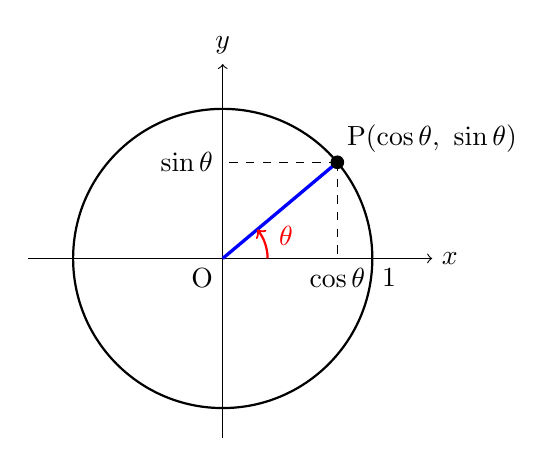
\begin{tikzpicture}[scale=1.9]
  \draw[->] (-1.3,0) -- (1.4,0) node[right] {$x$};
  \draw[->] (0,-1.2) -- (0,1.3) node[above] {$y$};
  \draw[thick] (0,0) circle (1);
  \coordinate (P) at (40:1);
  \draw[very thick,blue] (0,0) -- (P);
  \draw[dashed] (P) -- (P |- 0,0) node[below] {$\cos\theta$};
  \draw[dashed] (P) -- (0,0 |- P) node[left] {$\sin\theta$};
  \draw[->,red,thick] (0.3,0) arc (0:40:0.3);
  \node[red] at (20:0.45) {$\theta$};
  \fill (P) circle (1.3pt) node[above right] {$\mathrm{P}(\cos\theta,\ \sin\theta)$};
  \node[below left] at (0,0) {$\mathrm{O}$};
  \node[below right] at (1,0) {$1$};
\end{tikzpicture}
